\TOWRITE{NT/...}{Finalise}
\TOWRITE{ALL}{Proofread concept and approach pass 2}

\subsection{Concept and Methodology}\label{sec:concept_methodology}
\eucommentary{5-8 pages}


\subsubsection{Concept}\label{sec:concept}

\TODO{HF: We can probably remove some of the material here?}
\TOWRITE{}{Open with reproducibility?}
Open Science is the principle that science, in order to be most
\textbf{impactful} and \textbf{socially responsible}, should be done \textbf{publicly}, with as
much of the scientific process and products \textbf{accessible, reviewable,
and reusable} by as many members of the global community as possible.
In the modern age of computational science, almost all academic
fields, from humanities to social sciences to biology and astronomy
are presented with exciting opportunities for Open Science.  As more and
more research takes the form of code and/or data, the opportunity to
share, reproduce, and reuse scientific work is greater than ever, even
enabling new forms of \textbf{interdisciplinary collaboration}.

\TOWRITE{}{
define various forms of reproducibility
emphasize practicality
reiterate "automating existing practices"
}

At the same time as we share in these exciting opportunities, there
are corresponding challenges, technical and social, to making Open
and Reproducible Science a practical reality.  We face big questions: If a researcher
has code and/or data to publicise, how is that best done?  How do
researchers learn \textbf{best practices for Reproducible Open Science} in their field?  How do
previously disconnected fields benefit from each other's work as the
same computational challenges are faced again and again by different
communities?

These are the questions that guide \TheProject.
With so much research being done that wants to be Open and Reproducible,
how can we make Science

\begin{enumerate}
    \item as \textbf{easy} as possible to share and reproduce?
    \item as \textbf{useful} as possible to other researchers and the public?
\end{enumerate}

\noindent Our plan for \textbf{increasing the reproducibility of scientific results} can be summarised as:

\begin{enumerate}
\item improve and maintain \textbf{common software infrastructure} used for
  reproducing computational results,
\item develop the Jupyter ecosystem to improve capabilities to \textbf{better
  serve Reproducible Open Science},
\item \textbf{guide, validate, and demonstrate} our developments through
  collaboration with a wide variety of application domains,
\item enable students and researchers to perform Reproducible Open Science through
  \textbf{training and education}, and improving inclusiveness by focusing
  these on under-served and under-represented communities
\end{enumerate}

\medskip

\subsubsection{Reproducibility}\label{sec:concept}

Before describing the focus of the work that we propose here, we want to embed
this into the much wider context of reproducibility challenges.

We will exclude the challenges of reproducing \emph{experimental} data. Our
study starts at the point where such experimental data is available in digital
form.

We will focus on the challenge of computational reproducibility: can we carry out
the same data analysis, creation of figures and tables as they are presented in
a paper, at a later stage, and get to the same results?

Such tables and figures in a publication may be computed from the analysis of
some type of raw data which could originate an experiment, another publication,
a data base, post-processing of another data set or from executing computer
simulations.

% Where additional software, such as analysis scripts, input files
% and software for the simulation are needed, 

\subsubsection{Challenges of Reproducibility}

The challenges of such ``computational reproducibility'' include:
\begin{itemize}
\item Are the different processing steps for that data recorded? This could be
the order in which analysis scripts need to be executed -- for example to
compute intermediate results -- which will be turned into a figure in the last
step?

We will call this sequence of steps the \emph{workflow}. This workflow could be
archived -- for example -- through a \softwarename{README.txt} file, or scanned
pages of a hand-written laboratory notebook as a pdf file, or as a
machine-executable script (or a Jupyter notebook).

This is particularly challenging where software is used which can only be
controlled via a Graphical User Interface, as it may require manual recording
and description of the different clicks and steps in laboratory logbook.

\item Are all the scripts and configuration files (and more generally all
software) that is needed in this process known and archived? 

\item Where software is involved, have we recorded which version of that
software is needed (or was used)? If compilation is required, do we know which
compilers (and which version) and which additional dependencies are required?

\item Are there instructions how to obtain / compile the required dependencies,
and the software itself (in particular where this is about simulation based
science or more complex analysis and interpretation software tools)?

\item Where raw data is required, is this archived, accessible, and sufficiently
documented that the format is understandable?
\end{itemize}


\subsubsection{Reproducibility concept}

We can classify the reproducibility challenges listed above into different categories:

\begin{description}
\item[1. Workflow]: Are the processing commands (and their order)
correctly recorded? Do we know which part of the data set the analysis is meant
to be applied to? This is to a significant degree a question of the organisation
and documentation of the research process.

\item[2. Software environment]: Can we recreate the software environment that is
required to execute these commands?

\item[3. Importance]: Is the researcher convinced that investing effort into making
their work more reproducible is a worth while investment? This is a wide topic,
touching on expectations, existing cultures, lack of metrics that acknowledge
reproducibility efforts, and policies.

\item[4. Other]: There are other related topics, for example the challenge of
archival of (large) research data sets, of making the data FAIR, and the (for
some domains important) bit-wise reproducibility.
\end{description}

In this proposal, we start from practices that researchers increasingly adopt,
and which we argue are \emph{good reproducibility practices}. We propose to carry
out additional work to \emph{improve the toolset enabling this practice}.

To deal with the \emph{Workflow} challenges, we recommend to automate the
workflow steps as much as possible. In particular, the use of Jupyter Notebooks
to orchestrate the execution of commands seems effective~\cite{Beg2021}.
The use of the notebook is
perceived by many as an improvement of their research effectiveness because
it supports ``Thinking with Code and Data''~\cite{Granger2021}. A such, the
practice of using Notebooks (which helps improving research effectiveness) has
the very positive side effect of making the work more reproducible.


To deal with the \emph{Software environment} challenge, we recommend to follow
standard practices to describe software requirements. The \emph{focus of this
project is to extend the capabilities of the \repotodocker{} tool} to be able to
\emph{automatically create software environments} based on such software
requirement descriptions.

We can only partially address the \emph{Importance} challenge as this needs
concerted efforts from many stakeholders (such as employers of researchers,
research funders, publishers). However, we will offer training that advocates
the value of open science and that teaches existing best practice in 
effective computational science. The step from following such best practice to
making the work reproducible is -- given the Binder tools we want to develop
further here -- relatively small, or even possible without additional effort.

The \emph{Other} challenges are mostly outside the focus of this work
(although our proposal will also assist in reproducible and FAIR data
publishing, see for example Task \taskref{applications}{data-publishing}).


\subsubsection{Terminology and repository example}

For clarity, we define a few terms that we refer to through this proposal, and
illustrate this in the context of a education example repository
(https://github.com/fangohr/reproducibility-repository-example/
\cite{ReproducibilityRepositoryExample2022}).

We imagine that we have a publication that contains figure
\ref{fig:reproducibility-example-covid} as a result, and we want to archive and
make available the necessary information for others to reproduce that figure.

\begin{figure}
  \centering
  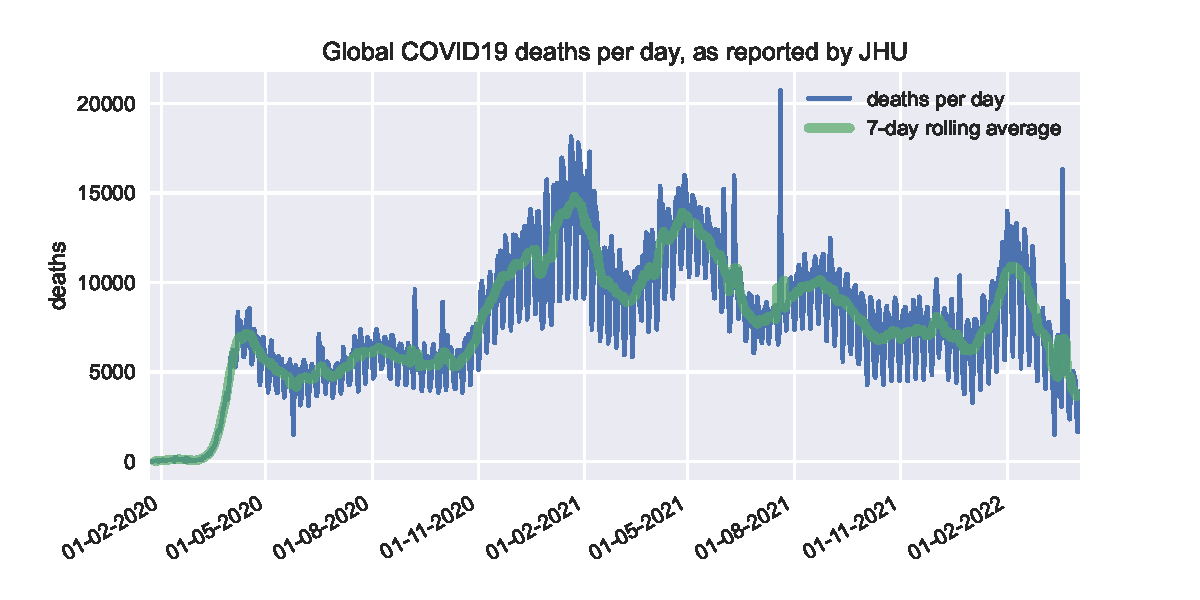
\includegraphics[width=0.8\textwidth]{images/figure1.pdf}
  \caption{Figure which can be reproduced in our explanatory repository example
    \cite{ReproducibilityRepositoryExample2022}. \label{fig:reproducibility-example-covid}}
\end{figure}

\begin{description}
\item[Repository] We refer to a \emph{repository} as a collection of files.

The \emph{purpose} of the repository in our context is to archive information to make
research results reproducible.

Such a repository could be a git repository (which could be hosted on github,
bitbucket, gitlab, or other services), but it could also just be a zip file of a
collection of files.

The repository could be made publicly available, for example through Zenodo,
Figshare, as an electronic supplementary to a publication, or through github.

It is not unusual that a larger number of files might be
organised in subdirectories within the repository.

Our example repository \cite{ReproducibilityRepositoryExample2022} contains the following files:

\begin{verbatim}
README.md - an overview of the content of the repository
figure1.ipynb  - notebook that creates figure1.pdf from the raw data
requirements.txt - software specification
time_series_covid19_deaths_global.csv  - raw data
\end{verbatim}

\item[Script] An machine executable file (for example a bash, Python, perl, file
or similar). Such scripts can execute data processing commands, and are often
part of a repository to make the (automatic) reproduction of results possible.

In our example, the necessary steps to create the figure from the raw data are
gathered in the notebook \texttt{figure1.ipynb}. 

\item[Notebook] A Jupyter Notebook. This is explained in \TODO{Add link to
relevant section}. In short, an executable document that can combine text, code
and computation results.

A Jupyter notebook can act like a script.

\item[Software specification] The software specification depends on the software
  tools used. In our example, the \texttt{requirements.txt} file contains
\begin{verbatim}
pandas==1.3.4
matplotlib==3.4.3
\end{verbatim}
to indicate that we need the pandas and matplotlib package with the respective
versions 1.3.4 and 3.4.3.

\item[Software environment] All the software that needs to be available and
  installed to execute the scripts and (and if desired) Jupyter notebooks.

\item[Project Binder] The Project Binder is described in Section
\ref{seq:project-binder}. It is part of the Jupyter ecosystem of tools, and
allows to convert a repository with Jupyter notebooks into an browser-hosted
environment, in which the notebooks can be executed interactively (and thus
results can be reproduced). \TODO{Point to binder section}

\item[Binder tools] The Bindertools consist of BinderHub (\TODO{See XXX}) and
\repotodocker{}. \TODO{@min - how do we summarise the role of BinderHub in one sentence?}

\item[\repotodocker] \repotodocker{} is a tool that can automatically create a
\emph{software environment} (currently within a Dotcker container) in which the
notebooks and scripts of a repository can be executed. \TODO{Point to dedicated section.}
\end{description}




\subsubsection{Project Jupyter and the surrounding ecosystem}
\label{sec:project-jupyter}

\begin{figure}[htb]\centering
  \includegraphics[width=0.9\textwidth]{use-cases-binder-logbook-solution.png}
  \caption{A typical use case for Jupyter notebooks in research.
            Image by Juliette Belin for the OpenDreamKit project, used under
            CC-BY-SA.}\label{fig:use-cases-binder}
\end{figure}

\noindent\textbf{Jupyter ecosystem as the root of \TheProject}

\TheProject has chosen to centre its efforts on the Jupyter software
ecosystem, in particular Binder and repo2docker.
Figure~\ref{fig:use-cases-binder} summarises a typical use
case of Jupyter Notebook and Binder;
both are described in more detail below.

The Jupyter notebook and Jupyter ecosystem are of increasing
importance in computational science and data science, in academia,
industry, and services. In addition to supporting high productivity of
researchers, they have great potential to push Open and Reproducible Science forward:
the notebook provides a complete description of a computational and
data science study (Step 1 in figure~\ref{fig:use-cases-binder}), and the notebook can -- in principle -- be turned
into a publication, or can be used to provide the required computation
for a part of a publication, such as a figure
(Step 2 in figure~\ref{fig:use-cases-binder}). Once the researcher has
specified what software is required to execute the notebook (Step 3
in figure~\ref{fig:use-cases-binder}), the study is completely
reproducible by anyone (Step 4 in figure~\ref{fig:use-cases-binder}).

In this way, the notebook \textbf{enables reproducibility} of complex tasks
with minimal additional effort on the user side.
The Binder project allows to execute such notebooks in
tailored computational environments; an aspect of reproducibility that
is not widely supported yet,
and a great opportunity for improving best practices in Open Science.

Furthermore, for users wanting to connect
to a local Jupyter notebook server on their machine, or to connect to
a server somewhere else on the Internet, the users only need a
web-browser to display and use the notebook regardless of the location
of the notebook server,
allowing computation to run anywhere from a local laptop to a remote supercomputer or in the cloud.
Because of these characteristics,
the Notebook is already planned to become an
important service on the European Open Science Cloud (EOSC) (for
example in \cite{panosc}),
and is an ideal component to use when building Open Science Services.

\medskip\noindent\textbf{Project Jupyter}

\emph{Project Jupyter} \cite{Jupyter}, which has grown increasingly popular in the scientific
computing community, has become the \emph{lingua franca} of interactive
computing in both academia and industry. The main goal of Project Jupyter
is to provide a consistent set of tools to improve researchers'
workflows from the exploratory phase of the analysis to the communication
of the results \cite{Kluyver2016}.

Split in 2014 from the \emph{IPython Project} \cite{IPython}, Jupyter has grown rapidly in
popularity and adoption both in the industry and academia. We estimate the user
base of the Jupyter notebook to be in the millions \cite{jupyter-grant}. Users range from data
scientists to researchers, educators, and students from many fields,
including journalists and librarians. In 2017, the Jupyter
team was awarded the \emph{ACM Software System Award}, an annual award that
honors people or an organization \emph{"for developing a software system that had a
lasting influence"}. Prior recipients include \emph{Unix}, \emph{TCP/IP}, and
the \emph{World Wide Web} \cite{acm-award}.

A large number of discrete software components make up Project Jupyter.
While these interact with one another, many can be installed separately
to serve various use cases. For this proposal, we loosely divide the
software involved into \emph{Jupyter core} developed under the guidance
of the developers who started the project, and the broader \emph{Jupyter
ecosystem} including software developed by third parties,
which may interact or build upon core Jupyter components.
Some of the components and concepts important to \TheProject are detailed below.

\begin{figure}[ht]\centering
  \centering
  \includegraphics[width=0.9\textwidth]{spectrogram_smaller.png}
  \caption{A notebook document in the Jupyter Notebook interface.}\label{fig:notebook-screenshot}
\end{figure}

\medskip\noindent\emph{Jupyter core}
\begin{itemize}
  \item The \textbf{Jupyter Notebook} is the flagship application of Project Jupyter.
  It allows the creation of notebook documents, containing a mixture of text and
  interactively executable code, along with rich output from running that code.
  Figure \ref{fig:notebook-screenshot} shows an open notebook including graphs
  from an audio processing example. Notebook documents are readily shareable,
  providing a popular way to describe and illustrate computational methods and
  tools. \TODO{We should update the notebook: (i) point to a github repo with it, and (ii) binder-enable it, and (iii) increase the pixel resolution of the screen shot.}
  \textbf{JupyterLab} is the new, modular, extensible client application
  for Jupyter notebooks, but the document format, server, and user model are the same.

  \item \textbf{Jupyter kernels} are the backend software which allow Jupyter to execute
  code in many different programming languages. The \textbf{IPython} kernel is
  the reference kernel, supporting the Python programming language, and is
  developed by the Jupyter core team. Kernels for other languages are maintained
  by third parties

  \item \textbf{JupyterHub} is a multi-user extension of the Jupyter Notebook.
  It runs on one or more notebook servers, for example at a research institution.
  Users can log in to author and run notebooks securely through their web
  browser, without needing to install any special software on their own
  computer.

\end{itemize}

\medskip\noindent\emph{Jupyter ecosystem}\label{jupyter-ecosystem}

While Jupyter is a large, distributed, coordinated project,
the wider community of Jupyter users develops a great deal of
software with Jupyter integration,
providing increased or domain-specific functionality,
building on top of Jupyter, or integrating core Jupyter components in some aspect.
We call this the \textbf{Jupyter ecosystem}.
The broader Jupyter ecosystem includes many more projects than we will describe
here, but a selection of projects which are relevant to
\TheProject includes:

\begin{itemize}
  \item \textbf{Binder} builds on JupyterHub to allow sharing executable
  environments along with data files and a description of the software components
  required to run the notebooks. When someone accesses a Binder repository,
  the service builds the computational environment on demand, allowing them to
  execute and modify a copy of the notebooks.
  \textbf{repo2docker} \cite{repo2docker} and \textbf{BinderHub} \cite{binder} are components of the Binder
  software. \TOWRITE{}{More here, as repo2docker is key}
\end{itemize}

\begin{figure}[ht]\centering
  \includegraphics[width=0.5\textwidth]{ipywidgets_example.png}
  \caption{An example of using two simple slider widgets to explore the
  parameter space of a function. The \texttt{@interact} decorator creates
  the widgets and connects them to the function.}
  \label{fig:ipywidgets-example}
\end{figure}


\subsubsection{Project Binder}\label{seq:project-binder}

\TOWRITE{}{Turn the following ideas into full sentences.}

\paragraph{Relationship to Jupyter}
\begin{compactitem}
\item Binder is part of Jupyter
\item Bindersubproject (within the Jupyter project) consists of
\begin{compactitem}
\item Repo2docker
\item BinderHub
\end{compactitem}
\item Binder project is operating within Jupyter ecosystem
\item But not confined to notebooks
\item Focus for this proposal is on \repotodocker{} part
\item \repotodocker{} solves software environment question in generic way
\end{compactitem}
\TODO{Add image that depicts this Jupyter/Binder relation ship}.

\paragraph{Basic functionality of Binder}
\label{binder-how-does-it-work}

\begin{compactitem}
\item Binder is \TOWRITE{}{what?} User entry point (for example on mybinder.org) is web interface \TODO{Add image of mybinder.org webpage?}
\item Binder is passed a URL from the user, for example a URL of a git repository with notebooks
\item Binder is asking \repotodocker{} to create a docker container in which the notebooks from the repository can be executed
\item \repotodocker{} searches the repository for specifications of software requirements (see \ref{repo2docker-supported-software-specifications}).
\item \repotodocker{} composes a Dockerfile that contains all the identified commands to install software
\item \repotodocker{} builds the Docker image based on the Dockerfile
\item \ldots \TOWRITE{}{Continue, and explain role of BinderHub and Kubernetes along the way}.
\end{compactitem}

\TODO{Explain: mybinder.org (service) is not binder (software)}

\paragraph{Supported software specification formats}
\label{repo2docker-supported-software-specifications}
\begin{compactitem}
\item Python packages (\softwarename{requirements.txt})
\item Conda packages (\softwarename{environment.yml})
\item \ldots
\end{compactitem}

\TOWRITE{}{}

\medskip
\paragraph{Binder for reproducibility}
\TOWRITE{}{}

\medskip
\noindent\textbf{Jupyter as a basis for web services}\\
Because the Jupyter notebook is a web-based application, it can be
deployed at computational facilities or in the cloud, and can function
as the basis for services exposing computational resources of all
kinds to researchers and the public.  Because Jupyter is
\textbf{interactive}, it enables making scientific results and
communications more interactive than static publications.  The
audience can follow their own initiative and ask their own questions
of published data without needing support from the publishing author,
greatly facilitating the \textbf{practicality of Open Science}.

\medskip
\noindent\textbf{Jupyter is generic}\\
\TheProject chose Jupyter because it is
Generic.  Jupyter makes no domain-specific or even language-specific
assumptions.  Any application where mixing description, code, and
results is valuable can make use of Jupyter.  This broad applicability
makes investment in the Jupyter ecosystem extremely effective, because
improvements to Jupyter can serve many communities simultaneously.

Jupyter is built from a collection of standard protocols and file
formats.  Jupyter is not just a single, monolithic piece of
software, but a description of how such software can be built.  The
result is the ability for a variety of communities and applications to
use components of Jupyter for their purposes, and/or reimplement pieces to
meet their needs.
%
For example:
\begin{enumerate}
\item The notebook file format is a well-specified JSON document,
  which can be interpreted by many systems.  This has facilitated the
  development of different services providing rendering of notebooks, e.g. the code
  hosting website GitHub, which renders notebooks for easy viewing by
  anyone, without Jupyter software.
\item The Jupyter protocol describes how execution is performed, which
  has enabled the development of over one hundred kernel
  implementations in dozens of languages\footnote{\url{https://github.com/jupyter/jupyter/wiki/Jupyter-kernels}}.
\item Output in the Jupyter protocol uses web-standard MIME types,
  enabling any possible format to be an output in a Jupyter notebook.
\item The JupyterLab extension system provides a system for building
  applications from Jupyter components and others.
\item The Jupyter Widgets provide a system for customizing and
  extending interactivity in Jupyter-based environments.
\end{enumerate}

The popularity of Jupyter, with millions of users and hundreds of open
source contributors, is an indicator of the value and impact of this approach.

\medskip
\noindent\textbf{Improvement to the Jupyter ecosystem}\\
The benefits of focusing our work on a mature system like Jupyter include:

\begin{itemize}
\item vibrant community ensures health and sustainability,
\item large existing user base maximises impact of contributions,
\item mature software ecosystem maintains quality software through
  industry standards such as version control, tests, continuous
  integration, stable release cycles, roadmaps, and user support.
\end{itemize}

The Jupyter community aims to be inclusive, and \TheProject fully
embraces and supports that approach.  Jupyter is inclusive across a number of axes.
By being applicable across numerous domains, Jupyter and \TheProject
encourage participation from individuals of various interests and
backgrounds, and has taken action to improve diversity in the project
by participating in ``Outreachy,'' a program of paid internships for
individuals from groups that face under-representation, systemic bias,
or discrimination.  Jupyter has also operated workshops focused on
training contributors from under-represented groups.  In being free,
public, open source software, Jupyter and \TheProject are accessible
to as many individuals as possible, and invites users and contributors
beyond origin, nationality, beliefs, orientation.  One area where
Jupyter has lacked in this regard is in the User Interface
accessibility, and we will help improve this in
% \taskref{core}{accessibility}
.  Additionally, the project will
focus some of its workshops in
% \taskref{education}{workshops}
on
under-represented communities.


\begin{figure}[ht!]\centering
  \includegraphics[width=0.6\textwidth]{images/notebook_components.png}
  \caption{The architecture of the Jupyter Notebook, kernels, and tools
        which operate on notebook files}
  \label{fig:notebook-architecture}
\end{figure}

\medskip
\noindent\textbf{Related projects}

\TOWRITE{}{The MyBinder.org federation}

\subsubsection{Methodology}\label{sec:methodology}

\textbf{Improving the robustness of reproducible environments (\WPref{reproducibility})}\\
Finally, we are explicitly allocating time in \WPref{core} for maintaining
Jupyter software, as well as new development
 % (\taskref{core}{maintenance}).
Maintenance is crucial to creating reliable, sustainable software,
but its cost is often swept under the rug in funding applications
because of the perceived pressure to focus on novelty.
Being up front and explicit about this cost is critical to the sustainability
of open source open science.

\medskip
\noindent\textbf{Broadening  (\WPref{impact})}\\
In addition to improving how successfully and how often tools like \repotodocker{} reproduce environments,
we aim to broaden the impact of the tools by making them useful in more contexts.
The existing software makes certain assumptions about where it will run,
made for the purposes of limiting maintenance scope of the Binder project.
As the project has matured, certain expansions of scope are appropriate,
as seen in the existing demand for new features in the project.

We further propose improvements to the wider Binder ecosystem
to expand the impact of the tools in more contexts to be useful to more researchers
and more institutions.
In particular, we have identified planned improvements:

\begin{itemize}
  \item Binder and its crucial software component \emph{repo2docker}
  \item relaxing Kubernetes assumption
  \item running on HPC
  \item more buildpacks
    % (\taskref{ecosystem}{r2d-and-binder}).

\end{itemize}

\medskip\noindent\textbf{Beyond the improvement to \TheProject tools
  (\WPref{applications}, \WPref{education})}\\
Beyond the improvement to the Binder tools for reproducility, we plan on
\begin{itemize}
\item Design, implementation, application, demonstration and
  evaluation of multiple demonstrators, that cover research fields such as
  \TOWRITE{}{photon and neutron science, geosciences},
  and also interests of participating SMEs (\WPref{applications}).
\item Producing \emph{training and education material} to disseminate
  the ability to do reproducible computational science using the tools
  we develop, among others (\WPref{education}).
\end{itemize}

\medskip
\noindent
\textbf{The science
  demonstrators}\label{sec:science-demonstrators-in-concept}\\

We describe the context and challenges for each demonstrator in this
section. The particular planned activities are shown in the
corresponding tasks in \WPref{applications}.\\


\TOWRITE{}{

1 page: National or international research or innovation activities
½ page: bringing together expertise and methods from different disciplines
½ page: social science and humanities - how do we integrate them, or why do we not need them
1 page: gender dimension. How taken into account in the research content (not the research team). Or justify why not relevant.
1 page: open science practices and implementation
1 page: research data management and management of other research outputs. (Also FAIR)

}
